
\chapter{Problem definition}

As discussed in the background section the U-Sem paradigm defines how the user modelling services has to be organized by orchestrating specific types of functional components. There is, however, little information about how this services and components are constructed and managed in practice. Currently, the only work done in that direction is the adoption of a workflow management system(RDF Gears) which facilitates the orchestration of components into user modelling services. 

Discovering the potential of Social media for user modelling \textbf{cite Brusilovsky07} , has led to an increased demand for U-Sem engineers to design and build many user modelling services. As a result engineers are constantly required to implement or adapt variety of functional components that are needed for the new services. Because of the lack of standardized approach for building and managing all these components each engineer is responsible to adopt his own approach. We believe that this process of building modelling services requires a lot of overhead work for engineers and can also potentially lead to increased amount of implementation errors. Therefore, in this work we investigate whether the current situation can be improved by introducing a user modelling server that is designed to support the process of creating and exposing the services to the users so that the overhead work of the scientists is limited and they can focus on the core of their work - the user modelling and analysis algorithms.

In order to be able to provide such system we, first, have to identify how engineers work and what are the tasks that require them to do a lot of overhead work and can be fully or partially automated. Next sections address the process that we used in order to identify the high level features that engineers can benefit most from.

\section{Requirements gathering}

In this section we aim to elicit the needs of the users and structure them into high-level system features that will later be designed and implemented.

\subsection{Stakeholders}

Stakeholders are the people that are have some kind interest in the project. They are the ones that will be affected by the project and thus they are the people that will be the source for the characteristics of the system we have to build. We identified the following as the main stakeholders of the project:  

\begin{itemize}
\item Scientists - people that develop algorithms and approaches for user modeling and analysis and allow other scientits and users to access them.
\item ImReal - system that want to use the services provided by the scientists and has its own requirements
\item RDFGears - provide the workflow engine and want to reuse some of the things.
\end{itemize}

\subsection{Interviews}

Once we had identified the stakeholders of the project we started to think how to extract the requirements from them. Literature suggest a wide variety of possible approaches []. However, there is one technique that proves to be really effective and it is the semi structured interviews \cite{Dieste}. In order to perform it we prepared some important questions that we wanted to know and then we did discussions \textbf{TODO}

\subsection{Identified features}

We analysed carefully all the raw information that we gather from the interviews and we identified several high-level features. We presented them to the stakeholders and after some discussions we ended up with the following final features that the system should provide: 

\begin{itemize}

\item \textbf{Simplified access to social media}
Scientist base a lot of their analysis on the information provided by users in the social media. However, each social media provides access through a special API. Currently, each user implements a component for retrieving the required data from each type social media. Providing feature that makes available to all scientists flexible components that can be configured to retrieve specific data from the different types of social media is considered a big benefit from the engineers because it will save them considerable time and efforts. They also will not need to know the specific details concerning each of the APIs. 

\item \textbf{Plug-in environment}
Engineers constantly build new services and improve and adapt existing one. Therefore, the system should facilitate the process of extending it by plugging in custom logic such as RDFGears functions and other functional components. Users should be able to manage(add/update/remove) this custom logic runtime(without restarting the system). This process should not affect the work of other users.

\item \textbf{Universal data storage} 
Many of the engineers build services that need to store various types of data(e.g. intermediate and final results). Currently, they are forced to manually set-up databases and program the components needed for interacting with each type of data. This usually not a trivial task, it requires time and knowledge and therefore, it resembles a big overhead to the engineers. Thus, they can be significantly benefited if the system provides a mechanism that enables storage and retrieval of arbitrary types of data.

 
\item \textbf{Integration with Hadoop}
The amounts of information that have to be processed in the system can sometimes be huge. Sometimes, it has to be processed by external Hadoop based systems. Currently, engineers have to manually manage the exchange the information to and from the Hadoop systems. Therefore, providing a mechanism that facilitates and standardises the process is also considered as a benefit for some engineers.

\end{itemize}

\section{Feature prioritization}

Because of the limited scope of this thesis work we are focusing on the features that will bring the most advantage for the engineers. In order, to do have to prioritize the requirements based on the impact they will provide. This process, however, is not trivial since each of the stakeholders has slightly different view on the benefits provided by each of the features that we already identified. Therefore, we performed a research in order to find an approach that can be applied in this situation.

Requirements prioritization is a relatively old research topic and there are numerous approaches that are available \cite{Moisiadis}. The most popular include Quality Function Deployment (QFD) the Analytical Hierarchy Process(AHP), the cost-value approach proposed by Karlsson, Wiegers' method, as well as a variety of industrial practices such as team voting, etc. However, literature also suggests that there is no perfect solution for this problem and the applicability of each approach depends heavily on the particular situation it is used.

For our project, we choose the analytic hierarchy process approach \cite{Lowe90} . This decision was based on the fact that it is especially suitable for prioritizing a small number of requirements\cite{Karlsson} and it is a proven and widely used \cite{Karlsson2}. In literature, as a disadvantage of this approach is considered the fact that it takes no account of interdependencies between requirements \textbf{Lowe90}. However, this issue did not affect the solution because the project high-level features are loosely coupled and they have little dependency between each other. 


\subsection{Features prioritization using AHP}
In the Requirements gathering section we identified 5 high-level requirements(features) that cover the main functionality of the system. In this step we are using the AHP's pairwise comparison method in order to assess the relative value of the candidate requirements. We asked a group of four experienced project members to represent customers views. We instructed them on the process and asked them to perform  pairwise comparisons of the candidate requirements based on their value(importance). Fig.. \textbf{Apendix 1} shows the form that they were asked to fill.

We let the participants to work alone, defining their own pace. We also allowed them to choose the order of the pair's comparison. Discussions were also allowed. When all participant finished the pairwise comparison, as advised in \cite{Karlsson} we had to make sure that the provided results are consistent. In order to do that we had to calculate the the consistency indices of the pairwise comparisons. According to \cite{Karlsson} values lower than 0.10 are considered acceptable and even values around .12 are commonly achieved in the industry and can also be considered acceptable. The calculation showed that two of the participants has indices higher than .23 which indicates serious inconsistencies \textbf{fff}. Therefore, we asked them to revise their answers and the results afterwards we measured values that are acceptable \textbf{ffff}.
 
 \begin{table}[h!]
  \begin{center}
    \begin{tabular}{| l | l | l | l | l |}
    \hline
    & Stakeholder 1 & Stakeholder 2 & Stakeholder 3 & Stakeholder 4 \\	 \hline
    Consistency ratio & 0.04 & 0.23 & 0.13 & 0.26 \\
    \hline
    \end{tabular}
  \end{center}
  \caption{The initial consistency ratios for each of the stakeholders.}
\end{table}


 \begin{table}[h!]
  \begin{center}
    \begin{tabular}{| l | l | l | l | l |}
    \hline
    & Stakeholder 1 & Stakeholder 2 & Stakeholder 3 & Stakeholder 4 \\	 \hline
    Consistency ratio & 0.04 & 0.12 & 0.13 & 0.11 \\
    \hline
    \end{tabular}
  \end{center}
  \caption{Consistency ratios for each of the stakeholders after refinement.}
\end{table}

Once we had achieved satisfying results we calculated the distributions. We outlined the candidate requirements in a diagram and presented the results to the project members. Each requirement's determined value is relative and based on a ratio scale. Therefore, a requirement whose value is calculated as 0.20 is twice as valuable as a requirement with a value of 0.10. Additionally, the sum of the values for all requirements equals 1. This means that a requirement with a value of 0.10 provides 10 percent of the value of all the requirements.

\begin{figure}[h!]
  \centering
      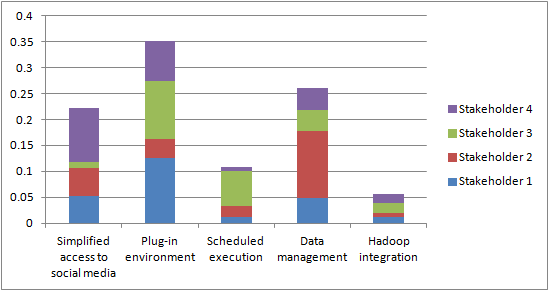
\includegraphics{requirements/value_diagram.png}
  \caption{The value distribution of the 5 requirements in the U-Sem project.}
\end{figure}


Finally, based on the provided results from the prioritization and the limited scope of this thesis we decided to further address the two features that will provide the most benefits for the users: "Plug-in Environment" and "Data Management". Next section sections cover each of the problems in details.

\section{Plug-in Environment}
\label{sec:problemDefPlugin}

During the initial interviews with scientists that are going to potentially use the system, we reviled that the nature of their work is very dynamic. In their day to day work they are expected to constantly improve and come up with new algorithms and approaches for user modelling. As a result, they are continuously producing new software code that implements these algorithms. After each production cycle, the program code has to be deployed into U-Sem so that it is available for testing, demonstration and evaluation purposes.

We also performed additional interviews with the scientist in order to reveal how this process is currently done, what are the problems they face with it and what are their expectations for the future system. Scientists reported that they have on their disposal only the capabilities of the workflow engine(RDFGears). However, it provides no functionality that enables to plug in custom logic on demand into the system and as a result, scientists are forced to "hardcode" their logic into the source code of the workflow engine. In this way, the software code implementing the algorithms becomes part of the workflow engine. We believe that this approach is error prone and brings a lot of discomfort to the scientists working with the system. The most important disadvantages of this approach include:

\begin{itemize}

	\item Adding new or modifying existing functionality requires a lot of time and knowledge since in order to do that one has to alter the source code of the workflow engine and basically, release a new version of it. This process requires advanced knowledge about each phase of the release process: checking out the source code from the software repository, putting the new source code in the appropriate place, building the system and finally, deploying it to the web server. Most of the time, all this knowledge is not required for the daily work of scientists and learning it may create a serious overhead and discomfort.
	
	\item In order to add/modify functionality one has to stop the web server where the system is deployed, replace the deployment entities of the system and start the server again. The problem with this approach is that during the time the server is down all other running services are unavailable. This is a major problem for everyone that is using the system during that time.
	
	\item Another major disadvantage is that, as a result of all the additional knowledge required, the training period for new scientists is significantly increased. This may easily cause project delays and missed deadlines.
	
	\item Multiple scientists adding/modifying functionality simultaneously may result in loss of functionality. Figure \ref{fig_vers_prob} illustrates the problematic scenario. As stated earlier, in order to add new functionality, scientists must first check out the source code of the system, make the changes and deploy the new version on the web server. However, if two scientist perform this process simultaneously then the new functionality provided by the first scientist will be lost when the second one deploys his version. 
	
	\begin{figure}[h!]
  \centering
  	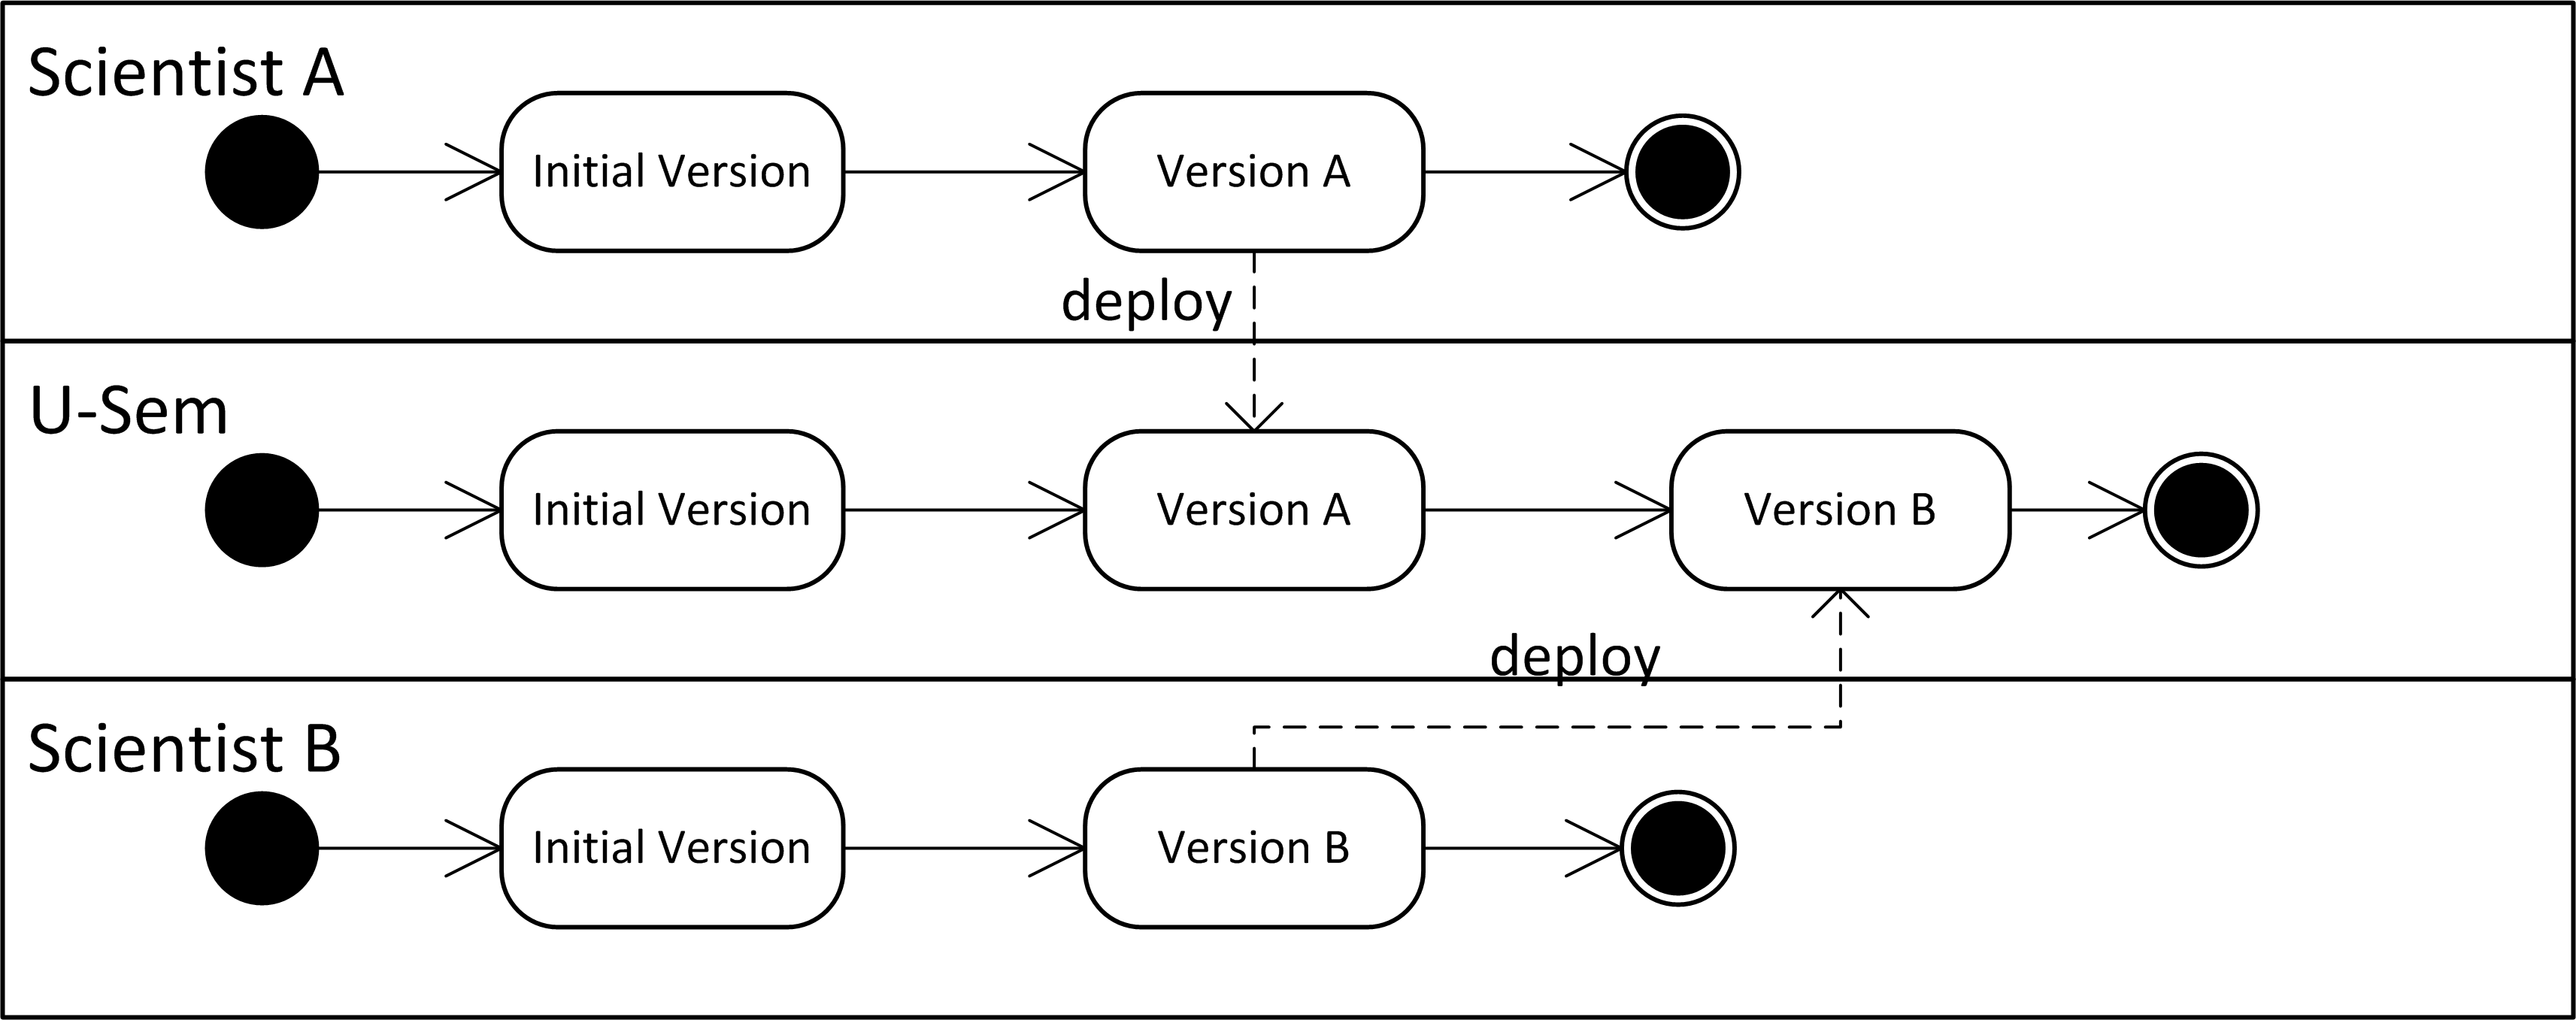
\includegraphics[scale=0.75]{plug-in/version_problem.png}
  \caption{State diagram illustrating the scenario where two scientists extend U-Sem simultaneously and the changes made by Scientist A are lost.  }
  \label{fig_vers_prob}
\end{figure}
	
	\item And last but not least, it is hard to verify what is the exact state of the system at any particular moment. Unless documented exclusively, it is not clear what additional functionality is added to the system. This problem becomes more serious when there are more people working on the project simultaneously and it is hard to track the changes in the system.
		
\end{itemize}

This approach also introduces one big disadvantage from software engineering perspective. The problem lies in the poor modularization of the system. In software engineering, modularization is considered as a key property for improving extensibility, comprehensibility, and reusability in software projects \cite{Parnas}. The most important aspect of a successful modular system is its information hiding capabilities \cite{Srivastava}. In our case, scientists can only rely on the modularization functionality provided by the Java language. However, its information hiding principles are only applied on class level, but not to the level of packages and JAR files. For example, it is not possible to restrict access to certain public classes defined in a package. The absence of such visibility control can easily lead to highly coupled, "spaghetti-like" systems \cite{Eder}. The consequences of this will become more and more clear with the time when the system grows in size, complexity and the number of engineers working on it increases. The most probable consequences include high development costs, low productivity, unmanageable software quality and high risk to move to new technology \cite{Cai}.

Having all these considerations in mind, we devised a complete set of requirements that presents the functional scenarios(functional requirements) and system qualities(non-functional requirements) that the proposed architecture has to provide. These requirements are also referred to into the evaluation section where we discuss how and to what extend the architecture satisfies each of them.

\section{Data Management}
\label{sec:problemDefStorage}

Our research showed that many of the services implemented by the engineers require data storage and retrieval in some form. The structure and semantics of the data varies greatly but we managed to classify the data in several groups:

\begin{itemize}

	\item \textit{Raw data} - Engineers reported that most of the analysis and modelling services they devised are based on the social media. Basically, they have to retrieve certain entries(e.g tweets from Twitter \textbf{foot note} ) which are the basis for the analysis. In certain cases engineers have to store this "raw data" locally. Usually, this is as a result of the fact that the retrieving the entities requires time and also the some social media APIs limit the number of entities you can get in certain amount of time \textbf{cite}. This makes the execution of workflows slow(the system has to wait to get the needed entries every time). Therefore, engineers are forced to store these entries an only make sure they are up to data prior to the execution of a workflow.
	
	\item \textit{User provided data} - Some services require information that is not available from the social media and has to be provided by the users of the system. For example, in certain usecases users has to fill in questioners and the results from later analysis is adjusted based on the answers provided by the users. It is infeasible to ask the users for that information every time that is why it has to be stored within the system.
	
	\item \textit{Intermediate results} - Some services consist of two phases. The first phase continuously calculates some intermediate representation of the raw data. In the second phase, on user request the final result is calculated based on the intermediate data. For example, \textbf{twinder}. Therefore, between the two phases the intermediate results has to be stored and later retrieved back.
	
	\item \textit{Ready user profiles} - Some services require that users has to be able to monitor how the results evolve over time. For example, in e-learning systems users want to be able to see how the knowledge of a certain person has changed after following a certain course and thus measure how helpful the course was for that person. Therefore, every time a service is executed the results has to be stored so that they can be later further analysed.
	
	\item \textit{System data} - Finally, many of the features of the system need to store some kind of information. For example, the multy-user sport has to store all kind information about the users of the system: user names, passwords, privileges, etc. The scheduling feature has to store information about the time each workflow has to be executed. 
	
\end{itemize}

Currently, the system does not provide any functionality to support users in defining workflows that require data operations. Each scientist is forced to create custom components that serve the particular requirements. However, we argue that this process wastes a lot of time, suffers from many downsides and problems:

\begin{itemize}
	\item \textit{Knowledge required} - designing and implementing components for dealing with persistent data is not a trivial job. It requires specific type of knowledge(\textbf{database, administration}). Many of the engineers building services have mathematical, statistical background are likely not to have in depth knowledge in the database field. These engineers have to learn this which can cause significant overhead and waste of time. Additionally, the fact that they are not professionals in the field may lead to problems and shortcomings.
	
	\item \textit{Server administration} - Most of the storing solutions require setting up a dedicated database server. These serves has to be hosted somewhere, maintained, backuped, etc. All these require a lot of effort and if every user has to do it, it will result in large amount of duplicated work and overhead. If engineers decide to use a shared database server then appears the question of who is responsible to manage it and ensure its security and privacy.
	
	\item \textit{Dynamic data structure} - It is expected that the structure of the stored data might change over time. When a database with fixed schema is used (like SQL) then every time the structure changes the engineers has to manually connect to the database and apply the changes manually. This can be really annoying, time consuming and error prone. Therefore, automating this process can save time to engineers and reduce the number of mistakes caused by carelessness. 
	
	\item \textit{Collaboration} - collaborations between engineers on data level is reported to be quite important and can save them a lot of time. Currently, there are no facilities available to support that requirement. Engineers have to organize this collaborations externally from the system. Additionally, this collaboration is hard to monitor and control.
	
	\item \textit{Low level queries} - Currently, most services use SQL databases. As a result, users have to deal with sql queries, which is considered as low level language \textbf{cite} and causes some overhead to the engineers especially the ones that are not familiar with it. Therefore users are for. Therefore, introducing some kind of higher level query language can be a big plus.
	
	\item \textit{RGL translation} - Generally available database solutions are not capable to deal with data in the RGL format introduces in RDFGears. Therefore, every single component that deals with persistent data has to translate the RGL values to values compatible with the databases solution and vice versa. Clearly, all this code is redundant and removing this responsibility from the engineers will save them time and efforts so that they can focus their attention to the core of their work.
	
	\item \textit{RDFGears and components with side effects} - Components that store data are components that have side affects. Generally, RDFGears is not designed to work with such components and some unexpected behaviour might be expected. Therefore, engineers building components with side effects and are not aware of the way RDFGears operate internally risk to introduce problems that are hard to detect.
	
\end{itemize}

In this thesis we aim to propose a solution that is capable to overcome these problems and save engineers a lot of time, efforts and prevent mistakes while dealing with persistent data.

\section{Conclusion}

\textbf{TODO}

\begin{thebibliography}{99}

\bibitem{Dieste}
Oscar Dieste, Natalia Juristo, and Forrest Shull, Understanding the Customer: What Do We Know about Requirements Elicitation?

\bibitem{Karlsson}
Karlsson, J., Ryan, K. (1997). A Cost-Value Approach for Prioritizing Requirements, IEEE Software September/October 1997, 67-74.

\bibitem{Karlsson2}
J Karlsson, C Wohlin, B Regnell - Information and Software Technology, 1998 - Elsevier

\bibitem{Moisiadis}
Frank Moisiadis, THE FUNDAMENTALS OF PRIORITISING REQUIREMENTS

\bibitem{Lowe90} Roper-Lowe, Gr C and Sharp, JA, The analytic hierarchy process and its application to an information technology decision, 1990

\end{thebibliography}